Our first task is to determine how to generate the vertices of the Stein complex $S$.
Each vertex $v$ of $X'$ yields a number of vertices in the Stein complex of $\pi'$, each of which map over $v$ it when we factor $\pi'$.
Here we have referred to $v$ as both the vertex of $X$ and the type 2 point in the image of $\pi'$ that the vertex corresponds to, and we do the same with the edges and 2--cells of $X'$.
According to the analysis in Section \ref{sec:3bound4}, a given vertex of $X'$ has at most two vertices in $S$ that will be difficult to find.
For $v$ a vertex of $X'$, introducing a vertex of $S$ over $v$ is based entirely on the behaviour of the circles that map over the regions incident to $v$.

In our first case, $v$ is an internal vertex.
There are four 2--cells $c_0,\dots,c_3$ of $X'$ that contain $v$ in their boundaries.
Put $C_i$ to be the collection of simplicial circles in $T'^*$ that project over $c_i$ as in the result of Algorithm \ref{alg:regularcircles}.
There are also four 1--cells $e_0,\dots,e_3$ where $e_i$ is the intersection of $c_i$ and $c_{i+1}$, indices computed modulo 4.
See Figure \ref{fig:vertexprime}.

An edge $E_0$ of $T'$ maps through $\pi'$ over $e_0$ and $e_3$, and $E_1$ maps over $e_1$ and $e_3$.
From Section \ref{sub:tridual} we know:
\begin{enumerate}
	\item $C_0\triangle \pd E_0^* = C_1$.
	\item $C_1\triangle \pd E_1^* = C_2$.
	\item $C_2\triangle \pd E_0^* = C_3$.
	\item $C_3\triangle \pd E_1^* = C_0$.
\end{enumerate} 
In the smooth case this is equivalent to finding cobordisms between sets of circles $C_i$ and $C_{i+1}$.
We say that an element $C_{i,k}$ of $C_i$ \emph{interacts} with an element $C_{i+1,j}$ of $C_{i+1}$ if $C_{i,k}\triangle C_{i+1,j}$ is either empty or exactly $\pd E_{\floor{i/2}}^*$.
Take the union of the $C_i's$ and partition it into subsets that such that any element of a subset interacts with at least one other element of that subset.
Call the set of subsets of $\bigcup_i C_i$ by $N(v)$ and call it the set of \emph{interactive elements} over $v$.
Every element of $N(v)$ adds a vertex to $S$ that is linked to the subset of $N(v)$ that spawned it.

In our second case, $v$ is a boundary vertex.
The analysis is exactly the same, except that there are only two 2--cells of $X'$ that are incident with $v$.
In $\C$, the last region incident to $v$ is $R_\infty$, so our analysis is simplified somewhat.
Otherwise, we perform the same steps as the internal case.

With the 0--cells of $S$ determined, we find 1--cells.
As with the vertices, the 1--cells of the Stein complex project over the 1--cells of $X'$.
Take $u$, $v$ vertices of $S$ adjacent over an edge $e$ of $X'$.
To find the associated edges of $S$, examine the sets of interactive elements over $u$ and $v$.
The shared circles within the elements of $N(u)$ and $N(v)$ tell us whether a pair of vertices are adjacent in $S$ as detailed in Algorithm \ref{alg:steinedges}.

Attaching the 2--cells is very similar to attaching the 1--cells.
A 2--cell of $S$ projects over a 2--cell $c$ of $X'$, and each 2--cell corresponds to a simplicial circle projecting through $\pi'$ over $c$.
The attachment is determined entirely by a cycle in the 1-skeleton of $S$, found in Algorithm \ref{alg:stein2cells}.

\begin{algorithm}[h]
	\caption{Finding vertices for the Stein complex}
	\label{alg:steinvertices}
	\KwData{a vertex $v$ of $X'$}
	\KwResult{the set $N(v)$ of sets of interacting circles near $v$}
	\Begin{
		$c_i\longleftarrow$ the 2--cells of $X'$ incident to $v$\;
		$C_i\longleftarrow$ the result of Algorithm \ref{alg:regularcircles} with input $c_i$\;
		$N(v)\longleftarrow\emptyset$\;
		\ForEach{circle $C_{0,k}$ in $C_0$}{
			$y\longleftarrow\{C_{0,k}\}$\;
			add each circle incident to $C_{0,k}$ to $y$\;
			add each circle incident to a circle incident to $C_{0,k}$ to $y$\;
			add $y$ to $N(v)$\;	
		}
	}
\end{algorithm}

\begin{algorithm}r[h]
	\caption{Finding edges for the Stein complex}
	\label{alg:steinedges}
	\KwData{an edge $e=(u,v)$ of $X'$}
	\KwResult{the set $N(e)$ of pairs $(U,V)$ with $U\in N(u)$ and $V\in N(v)$ such that $U$ and $V$ are adjacent over an edge of $S$}
	\Begin{
		$N(u), N(v)\longleftarrow$ the results of Algorithm \ref{alg:steinvertices} with inputs $u$, $v$\;
		$N(e)\longleftarrow\emptyset$\;
		\ForEach{element $U$ of $N(u)$}{
			\ForEach{element $V$ of $N(v)$}{
				\If{$U\cap V\neq\emptyset$}{
					add $(U,V)$ to $N(e)$\;
				}
			}	
		}
	}
\end{algorithm}

\begin{algorithm}[h]
	\caption{Finding 2--cells for the Stein complex}
	\label{alg:stein2cells}
	\KwData{a 2--cell $c$ of $X'$ with $\{v_0,\dots,v_k\}=\pd c$}
	\KwResult{the set $N(c)$ of cycles $\{V_0,\dots,V_k\}$ where $V_i$ is in $N(v_i)$ such that a 2--cell is attached over $\{V_0,\dots,V_k\}$ in $S$}
	\Begin{
		$C\longleftarrow$ the result of Algorithm \ref{alg:regularcircles} with input $c$\;
		$N(v_i)\longleftarrow$ the result of Algorithm \ref{alg:steinvertices} with input $v_i$\;
		$N(c)\longleftarrow\emptyset$\;
		\ForEach{simplicial circle $C_j$ of $C$}{
			$N_j\longleftarrow\emptyset$\;
			\ForEach{integer $i$ in $[0,k]$}{
				\ForEach{element $V_i$ of $N(v_i)$}{
					\If{$C_j\in V_i$}{
						add $V_i$ to $N_j$\;
					}	
				}			
			}
			add $N_j$ to $N(c)$\;
		}
	}
\end{algorithm}

\begin{figure}
	\centering
	\captionsetup{justification=centering}
	\caption{A vertex in $X'$ and the circles that map over incident 2--cells}
	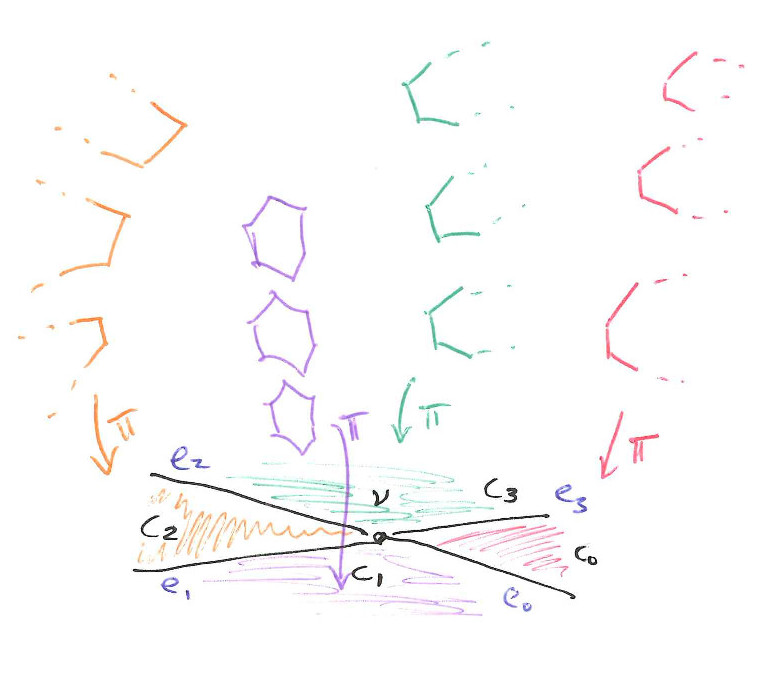
\includegraphics[height=4in]{figures/vertexprime.jpg}
	\label{fig:vertexprime}
\end{figure}